
% \picinclude{./050-059/p_s050.jpg} 
Verlangen zu tragen, daß Gott und Christus in ihren Herzen
und Leibern wohne, aus daß sie Tempel Gottes? würden. Denn
der Wostel sagt: ,,Gott wohnet nicht in Tempeln mit Händen
gemacht'' (Act. 7, 48). Weil man aber diese Stätten nun einmal
heilig hielt, so fand man ez- schrecklich, wenn man etwas dagegen
sagte. A18 ich inZ Turmhauß kam, waren nicht mehr altz 11 Zu-
hörer dort, und der Priester hielt ihnen die Predigt. Alß nun
in der Stadt bekannt wurde, ich sei im Turmhause, so füllte sich
daßselbe bald mit Menschen. Alk- der Priester, der an dem Tage
zu predigen hatte, geendet hatte, hieß er den andern Priester, der
mich aufgefordert hatte zu kommen, mich auf die Kanzel führen,
aber ich ließ ihm sagen, ich brauche nicht auf eine Kanzel zu
steigen. Darauf ließ, er mir wieder sagen, er wünsche aber, daß
ich sie befteige, weil dort ein besserer Platz sei, an dem mich die
Leute sehen könnten. Ich ließ ihm darauf sagen, man sehe mich
gut genug, da wo ich sei, ich sei nicht gekommen, solche Stätten
noch aufrecht zu erhalten und ihr Bestehen und den Handel, der
damit getrieben wird. Alk- ich dieö gesagt hatte, fingen sie an,
böse zu werden und sagten: ,,Da8 sind die falschen Propheten
der letzten Zeiten«. Diese Rede Verletzte etliche und sie murrten
darüber; nun stand ich auf und hieß alle ruhig sein; ich stieg
auf einen hohen Stuhl und erklärte ihnen, woran man die falschen
Propheten erkenne, und daß sie schon gekommen seien; und dann
zeigte ich ihnen im Gegensatz dazu die wahren Propheten, Christus-
und die Apostel. Ich wieß sie alle an ihren inneren Lehrer,
Christue, der sie von der Finsterniö zum Lichte führen könne.
Nachdem ich ihnen verschiedene Schriftstellen erklärt hatte, wies
ich sie auf den Geist Gottes in ihren Herzen hin, durch welchen
sie zu ihm kommen könnten und erkennen, wer die falschen
Propheten seien. Nachdem ich so ein reiches Wirken unter ihnen
gehabt hatte, zog ich im Frieden von dannen ....
Hierauf kam ich nach Pickering, wo die Richter im Turm-
hauö ihre Sitzungen hielten; Ftiedenztichtet Robinson war Vor-
sitzender. Ich hatte zur gleichen Zeit eine Versammlung im
Schulhaus und viele »Fromme« und Priester wohnten ihr bei
und stellten allerlei Fragen, die zu ihrer Zufriedenheit beantwortet
wurden. ES war gerade die Zeit der Gerichtösit-zungen, und da
wurden auch vier Oberkonstabler bekehrt. GS kam Richter Robin-
son zu Ohren, daß der Priester, den er allen andern Priestern


% \picinclude{./050-059/p_s051.jpg} 
Erlebnisse im Gefängnis zu Terby usw. 51
oorzog, besiegt und überzeugt worden war. Wir gingen nach
der Versammlung in eine Herberge; Richter Robinson’s Priester
war sehr bescheiden und lieb und wollte sogar durchaus mein
Essen bezahlen, was ich aber nicht zuließ. Dann bot er mir sein
Turmhaus an, um darin zu predigen, aber ich lehnte es ab und
erklärte ihm und den andern, daß ich eben gekommen sei, um die
Leute oon diesen Dingen ab und zu Christus zu bringen.
Am folgenden Morgen ging ich mit den vier Konstablern und
andern, um Richter Robinson zu besuchen, der mir unter der
Türe seines Zimmers entgegenkam. Jch sagte ihm, ich könne ihm
keine menschliche Ehre erweisen; er sagte, er sehe nicht aus das.
Jch ging nun mit ihm ins Zimmer und tat ihm den Unterschied
zwischenswahren und falschen Propheten dar, und wie die wahren
höher stehen als die falschen, und richtete seinen Sinn aus
Christum seinen Lehrer. Jch deutete ihm die Gleichnisse, und
wie es sich mit der Grwählung und Verwersung verhalte, wie
man in der ersten Geburt in der Verwersung sei und in der
zweiten in der Grwählung. Ich zeigte ihm, wer die Verheiß-ungen
Gottes habe und wen sein Gericht verdamme. Gr gab alles zu
und war so offen für die Wahrheit, daß, wenn ein anderer an-«
wesender Richter eine kleine Ginwendung machen wollte, er ihn
belehrte. Beim Fortgehen sagte er, ich tue sehr gut, diese mir
von Gott verliehene Gabe zu gebrauchen. Gr nahm den obersten
Konstabler beiseite und wollte ihm etwas Geld siir mich geben,
weil er nicht wollte, daß ich in ihrer Gegend irgend welche Aus-
gaben habe; aber sie sagten ihm, daß ich nicht dazu zu bringen
sei, etwas anzunehmen. Jch schätzte seine Freundlichkeit, das
Geld jedoch lehnte ich ab.
Jch zog im Lande umher und der Priester, der mich Bruder
genannt hatte, zog mit mir. Als wir in eine Stadt kamen, wo
wir im Sinne hatten etwas zu essen, läuteten die Glocken.
Jch fragte, warum sie läuten; man sagte mtr, sie läuten für mich,
damit ich im Turmhaus predige. Bald daraus trieb es mich
dorthin. Als ich kam, sah ich die Leute auf dem Turmhausplatze
versammelt; der alte Priester wollte, daß ich ins Turmhaus gehe,
  ich sagte, es sei nicht nötig. Ge besremdete die Leute, daß
ich nicht in das gehen wollte, das sie ,,Goiteshaus« nannten. Jch
stellte mich auf den Platz des Turmhauses und erklärte den Leuten,
ich sei nicht. gekommen, ihre göizendienerischen Tempel ausrecht
 


% \picinclude{./050-059/p_s052.jpg}
zu erhalten, noch die Priester mit ihren Zehnten, Zulagen, Ab-
gaben und Pfrtinden, noch ihre jüdischen und heidnischen Zere-
monien und Traditionen; denn die gelten mir alle nicht?-. Jch er-
klärte ihnen, dieses Stück Boden sei nicht heiliger, ale irgend ein
anderes Stück Land. Jch zeigte ihnen, daß die Apostel, wenn
sie in die Synagogen und die Tempel der Juden gegangen seien,
die ja Gott selber sogar vorgeschrieben habe, so sei ez nur ge-
schehen, um die Leute davon Iabzubringen und von den Opfern
und Zehnten und den habsüchtigen Ptiestem jener Zeit. Und
die, welche zur Wahrheit belehrt wurden und an den von den
Aposteln gepredigten C-hristuö Hglaubten, hätten sich nachher in
den Wohnhäusern versammelt. Ich sagte ihnen, daß alle, welche
Christus, daß Wort deö Lebenß, predigen, eö umsonst tun sollen
wie die Apostel, und wie Christus eß geboten habe. So war ich
gesandt worden von Gott dem Herrn Himmels und der Erden
umsonst zu predigen und die Leute von diesen äußeren Tempeln
mit Händen gemacht, worin Gott nicht wohnt, abzubringen, damit
sie erkennen, daß ihre Leiber Tempel Gottes werden sollen. Jch
mußte die Leute abbringen von ihren jüdischen Zeremonien, aber-
gläubischen und heidnis chen Gebräuchen, Traditionen und Menschen-
satzruigen, von der Lehre all der Mietlinge, die Zehnten nehmen
und große Psründen, die um Bestechung predigen und für Geld
weiösagen, die gar nicht von Gott und von Christus gesandt
sind, wie sie ja selber bekennen, wenn sie sagen, sie haben nie
die Stimme Gotteß noch Christi vernommen. So ermahnte ich
denn die—Leute, abzulassen von alle dem, und wieß sie auf den
Geist und die Gnade Gottetz hin, welche inwendig in ihnen sind,
und auf daß Licht Jesu in ihren Herzen, aus daß sie dazu kommen
möchten, C-hristum zu kennen, der sie umsonst lehre und ihnen
Rettung bringe und ihnen die Schrift öffne. Alleö war ruhig
und viele wurden gewonnen, der Herr sei gepriesen.
Jch kam daraus in eine andere Stadt, wo wieder eine große
Versammlung war; der vorhin erwähnte Priester begleitete mich
und allerlei ,,Fromme« kamen dazu herbei. Ich saß mehrere
Stunden auf einem Heuschober und sagte nichte, denn sie sollten
nach Worten hungern. Die ,,Frommen« kamen immer wieder
zu dem alten Priester und fragten ihn, wann ich beginnen werde
zu reden. Er hieß sie warten und sagte ihnen, das Volk habe
immer lange gewartet, bis Christus gesprochen habe. Schließlich


% \picinclude{./050-059/p_s053.jpg} 
Erlebnisse im Gefängnis zu Derby usw. 53
trieb mich der Herr zu reden, und sie wurden von der Kraft deö
Herrn erfaßt; das Wort detz Lebens erreichte sie und es- geschah
eine allgemeine Bekehrung unter ihnen.
Ich zog weiter; der alte Priester und einige andere waren
mit mir. Unterwegß riesen ihn ein paar Leute an: ,,Mr. Bones,
wir sind euch Geld schuldig für Zehnten; kommt doch und nehmt
eZ!« Aber er wehrte mit der Hand ab und sagte, er habe genug,
er wolle nichtß davon, sie sollten ez nur behalten; und er prieß
Gott, daß er solcheö sagen konnte. Schließlich kamen wir zu dem
Turmhauß dieses- alten Priesters im Nioor; alß wir eingetreten
waren, ging er vorausz und öffnete die Kanzeltür, aber ich sagte ihm,
ich würde nicht hineingehen. Das Turmhauß war stark bemalt;
ich sagte ihm und den Leuten, die dabei waren, daß gemalte Tier
(Offb. 17, 3.) habe ein gemalteß Haus. Dann erklärte ich ihnen die
Entstehung aller dieser Häuser und ihre abergläubischen Gebräuche;
ich zeigte ihnen, daß die Apostel nicht in die Tempel gegangen
seien, um diese aufrecht zu erhalten, sondern um die Leute zu
Christuö, dem wahren Gut, zu führen; ich zeigte ihnen den wahren
Gotte?-dienst, den Christus gegründet hat; ich zeigte den Unter-
schied zwischen Ehristuß dem wahren Weg und allen verkehrten
Wegen, indem ich ihnen die Gleichnisse deutete und sie von der
Finsternitz zum wahren Lichte wieö; damit sie durch dasselbe sich
selbst erkennen möchten und ihre Sünden und ihren Erlöser und
durch den Glauben an ihn erlöst würden von ihren Sünden .....
Nun kam ich nach Eranstick, zu Hauptmann Purßloe und
Friedenßrichter Hotham, die mich beide freundlich empsingen, weil
sie sich freuten, daß die Kraft des Herrn erschienen war und daß
die Wahrheit sich auzbreitete und so viele sie aufnahmen, und daß
Frichen?-richter Robinson so freundlich gewesen war. Hotham
sagte, wenn Gott nicht diese Anschauungen von Licht und Leben
hätte kund werden lassen, so wäre daß ganze Land von den
Rantern überschwennnt worden und alle Richter des- Landeß mit
allen ihren Gesetzen hätten ihnen nicht zu wehren vermocht. ,,Denn«,
sagte er, ,,wenn sie auch gesagt und getan hätten, was- wir ihnen
befehlen, so hätten sie doch nicht von ihren Wisichten gelassen.
Aber eure Grundsätze der Wahrheit werfen alle ihre Grundsätze
und daß, worauf sie die ihrigen gründen, über den Hausen«.
Darum war er so froh, daß Gott diese Grundsätze des Leben-3
und der Wahrheit hatte durch mich kund werden lassen ....


% \picinclude{./050-059/p_s054.jpg} 
Als am folgenden Tage die Freunde mich verlassen hatten,
reiste ich allein weiter und verkündete den Tag des Herrn überall,
wohin ich kam, und ermahnte zur Buße. Eines Abends kam ich
in die Stadt Patrington, und während ich durch die Stadt ging,
ermahnte ich sowohl die Priester als das Volk Buße zu tun und
sich zum Herrn zu bekehren. Gs wurde finster, ehe ich ans Ende
der Stadt kam, und eine große Menge hatte sich um mich ver-
sammelt, während ich das Wort des Lebens verkündete. -- Als
ich meine Ausgabe erfüllt hatte, ging ich in eine Herberge und
verlangte Unterkunft für die Nacht, aber sie wurde mir verweigert.
Daraus bat ich um etwas Fleisch und Milch, ich wolle es bezahlen;
aber auch das wollte man mir nicht geben. So verließ ich die
Stadt; einige junge Leute kamen hinter mir drein und fragten
mich, was es neues gebe. Jch hieß sie Buße tun und Gott
fürchten. Als ich eine Strecke weiter gegangen war, kam ich wieder
an ein Haus und bat, man solle mir etwas Fleisch und Milch
geben und Nachtherberge, gegen Bezahlung; aber sie schlugen es
mir ab; dann ging ich zu einem andern Haus und verlangte das-
selbe; aber sie wiesen mich ebenfalls ab. Jnzwischen war es so
dunkel geworden, daß ich die Landstraße nicht mehr sehen konnte;
ich endeckte einen Wassergraben und schöpfte etwas Wasser um
mich zu erfrischen; dann überschritt ich den Graben und da ich
von der Reise müde war, setzte ich mich unter einen Ginsterstrauch
und wartete bis es Tag war. Mit Tagesanbruch erhob ich mich
und ging weiter. Hinter mir drein kam ein Mann mit einer
Heugabel, der schritt neben mir her bis zu einer Stadt, und
noch ehe die Sonne ausgegangen war, hatte er diese Stadt und
die Polizei gegen mich ausgehetzt; ich verkündete Gottes ewige
Wahrheit unter ihnen und warnte sie vor dem Tag des Herrn,
der kommen würde über alle Sünde und Ungerechtigkeit, und er-
mahnte sie, Buße zu tun. Mer sie.griffen mich und brachten
mich nach Patrington zurück, etwa drei Meilen weit, und be-
wachten mich mit Stöcken, Heugabeln und Hellebarden. Als ich
nach Patrington kam, war die ganze Stadt in Aufruhr. Die
Priester und das Volk berieten sich zusammen; so konnte ich
ihnen abermals das Wort des Lebens verkünden und sie zur Buße
ermahnen. Endlich nahm mich einer der »Frommen«, ein guter
Mann, mit in sein Haus, wo ich mich an etwas Brot und Milch
erlabte, denn ich hatte seit mehreren Tagen nicht-3 gegessen. Dann


% \picinclude{./050-059/p_s055.jpg} 
Erlebnisse ini Gefängnis zu Derby usw. 55
schleppten sie mich etwa neun Meilen weit zu einem Richter.
Als wir nahe bei dessen Haus waren, kam einer hinter uns her
geritten und fragte mich, ob ich der sei, der verhaftet worden
war. Ich fragte, warum er es wissen wolle; er sagte, es ge-
schehe in keiner bösen Absicht; da sagte ich ihm, daß ich es
sei; darauf ritt er voraus zum Richter. Meine Begleiter sagten,
hoffentlich sei der Richter nicht betrunken, wenn wir zu ihm
kämen; denn er pflegte schon frtihmorgens betrunken zu sein.
Als ich vor ihn trat und meinen Hut nicht abnahm und ihn mit
Du anredete, fragte er den, welcher uns oorgeritten war, ob ich
verrückt sei, aber er sagte ihm, nein, es sei mein Grundsatz. Jch
ermahnte den Richter, Buße zu tun und sich zum Licht zu be-
kehren, mit dem Christus ihn erleuchtet, damit er durch dasselbe
alle seine bösen Worte und Taten erkennen möge, und zu Christus
zurückzukehren, solange es noch Zeit sei. ,,Ja, ja«, sagte er, ,,das
Licht von dem im dritten Kapitel des Johannes gesprochen wird-«.
Joh bat ihn, er möge doch auf dieses Licht achten und ihm ge-
horchen. Während ich ihn ermahnte, legte ich ihm die Hand auf,
und er ward übernommen von der Kraft des Herm und die
Wächter waren bestürzt. Er führte mich nun in ein kleines Gemach,
um zu untersuchen, was ich von Briefen und Schriften in der
Tasche habe; ich wies ihm meine Kleider und zeigte ihm, daß
ich keine Briefe bei mir hatte; er sagte, man sehe an meiner
Wäsche, daß ich kein Landstreicher sei, und ließ mich frei. Jch
ging mit dem Mann, der vor uns hergeriiten, nach Patrington
zurück, denn er lebte daselbst. Als wir ankamen, wünschte er, ich
solle eine Versammlung auf dem Hauptplatz halten, aber ich sagte
es sei nicht nötig, sein Haus genüge. Gr wollte, daß ich zu Bett
gehe oder mich doch aufs Bett lege; dies wünschte er namentlich,
damit er sagen könne, man habe mich in oder doch wenigstens
auf einem Bett gesehen; denn es ging das Gerücht, ich wolle
in keinem Bett schlafen, weil ich damals oft im Freien über-
nachtete. Als der Erste Tag kam, ging ich ins Turmhans
und verkündete dem Priester und dem Volk die Wahrheit; und
die Leute taten mir nichts, denn die Kraft Gottes war über sie
gekommen. Gleich nachher hatte ich eine große Versammlung in
dem Hause des Mannes, der mich beherbergte, und viele wurden
von Gottes ewiger Wahrheit überzeugt und sind derselben treu
geblieben bis aus den heutigen Tag. Sie bereuten es sehr, daß


% \picinclude{./050-059/p_s056.jpg} 
sie mich nicht aufgenommen und beherbergt hatten, als ich zuerst
bei ihnen gewesen war .......


%%%%%%%%%%%%%%%%%%% Kapitel 5. %%%%%%%%%%%%%%%%%%%%%%%%%%%%%%

\chapter[Quäkerischen Weltmission]{Quäkerischen Weltmission}

\begin{center}
\textbf{Christus in uns. Erkenntnis der Quäkerischen Weltmission. Das
Haus Richter Fells in Swarthmore; der Pöbel von Ulverstone.
Rechtfertigung vor dem Gericht in Lancastre.}
\end{center}



\begin{floatingfigure}[3]{4cm}
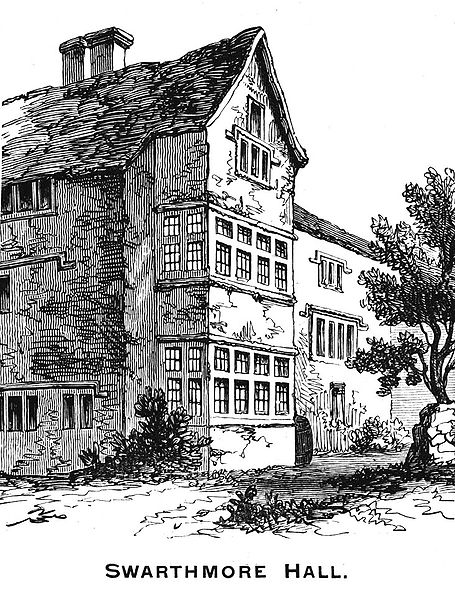
\includegraphics[width=0.20\textwidth]{./pics/swarthmore_hall.png}
\label{bild:swarthmoor} 
\end{floatingfigure}



Wir zogen durch Nottinghamshire nach Lineolnshire .....
Hier kam zu einer unserer Versammlungen ein Mann und erhob eine
falsche Anklage gegen mich; er verbreitete überall daö Gerücht, ich
habe gesagt, ich sei Christus-, was gänzlich falsch war. Al-? ich dann
nach Gainßborough kam, wo einer der Freunde auf dem Markt-
platz die Wahrheit verkündet hatte, fand ich die ganze Stadt und
alle Marktleute in Aufruhr. Jch ging inß Haus eineö Freunde?-,
und daß Volk drängte sich hinter mir drein, biz das Haus ganz
voll war von »Frommen«, Giferern und Pöbel; da kam jener
falsche Verleumder herein und klagte mich öffentlich vor allen an,
ich hätte gesagt, ich sei Christuß, und er habe Zeugen, es zu be-
weisen. Das brachte die Leute so in Wut, daß man Miihe hatte,
mich vor ihnen zu schützen. Da trieb mich der Geist dez Herrn
aus einen Tisch zu stehen und in der ewigen Kraft dez Herrn
den Leuten zu verkünden, daß Christuö in ihnen sei, etz sei denn,
daß sie Verdammte seien; und daß eß Christuö, die ewige Kraft
Gottes sei, welche jetzt auß mir zu ihnen rede, nicht ich sei Christus;
die Leute waren im allgemeinen befriedigt außer jenem »Frommen«
und einigen falschen Zeugen. Jch nannte diesen Ankläger Judaö,
und es trieb mich, ihm zu sagen, daß das Ende deö Judaß auch
das seine sein werde; solches- lasse ihm der Herr durch mich sagen.
Dez Herrn Macht kam über alle und beruhigte die Gemüter der
Leute und sie gingen in Frieden fort. Jener Judaß aber machte
sich davon und erhenkte sich und man steckte einen Pfahl in sein
Grab. Daraufhin erhoben die bösen Priester eine Verleumdung
gegen unö und streuten aus, ein Quäker habe sich erhenkt in
Lineolnshire. Diese Lüge ließen sie drucken und verbreiten und
hänften so Sünde auf Sünde. Mer wir und die Wahrheit wurden
nicht davon getroffen; denn jener war so wenig ein Quäker als
der Priester, der solcheß gedruckt hatte; vielmehr war eögeiner


% \picinclude{./050-059/p_s057.jpg} 
Christus in uns. Erkenntniz der Quükerischen Weltmisfion usw. 57
ihrer eigenen Leute. Aber trotz dieser argen Lüge, mit welcher der
Gegner beabsichtigthatte, unß zu verleumden und die Leute von
der von unß verkiindeten Wahrheit abzukehren, nahmen doch viele
in Lineolnshire daß Evangelium an, da sie von der ewigen Wahr-
heit überzeugt waren und sich zu Füßen deß himmlischen Herm
setzten ......
Wir zogen nun wieder .... über Warmßworth . . . Bably,
Doneaster .... nach Tickhill, wo an einem Ersten Tage die
Freunde der Gegend sich versammelten, und eß herrschte durch
Gottes Macht eine tiefe Zerknirschung in der Versammlung.
Jch verließ die Versammlung, da Gott mich trieb inß Turmhauß
zu gehen. Alß ich dorthin kam, fand ich den Priester und saft
alle Gemeindeältesten im Chor beisammen. Jch ging zu ihnen
und hub an zu ihnen zu reden, aber sie sielen sogleich über mich
her, und ein Priester nahm seine Bibel und schlug mich damit
inß Gesicht, so daß ich heftig blutete im Turmhauß; daß Volk
schrie: ,,Hinauß mit ihm auß der Kirche!« Und alß sie mich hinauß
gebracht hatten, prügelten sie mich und warfen mich zu Boden
und über eine Hecke; hernach schleppten sie mich durch ein Hauß
aus die Straße; sie warfen mich mit Steinen und schlugen mich,
während sie mich Vorwärtß tissect, so daß ich über und über mit
Kot beschmiert war. Sie nahmen mir den Hut, den ich nicht
mehr wieder bekam. Alß ich jedoch wieder auf den Füßen war,
verkündete ich ihnen daß Wort deß Lebenß und zeigte ihnen, wo-
hin ihre Lehre sie führe und wie sie daß Christentum entehrten. Nach
einer Weile ging ich wieder in die Versammlung zurück zu den
Freunden. Und alß die Priester und die Leute am Hause vorbei
kamen, ging ich mit einigen Freunden hinauß in den Hof und
redete zum Priester rmd den Leuten. Der Priester verhöhnte
unß und nannte unß ,,Quäker«. Aber die Macht deß Herrn
kam dermaßen über sie und daß Wort deß Lebenß wurde ihnen
so überzeugend und eindringlich verkündet, daß der Priester selber
zu zittern begann und einer sagte: »seht wie der Priester zittert
und bebt, er wird auch ein Quäker«. Alß die Versammlung zu
Ende war, gingen die Freunde sort, und ich ging, ohne Hut,
nach Balby, etwa sieben bis acht Meilen weit. Die Freunde
wurden an dem Tage dergestalt von dem Priester und seinen
Anhängern mißhandelt, daß einige Friedenßrichter, alß sie davon
hörten, kamen und ein Verhör in dieser Stadt anstellten, um


% \picinclude{./050-059/p_s058.jpg} 
58 Kapitel lt.
die Sache zu untersuchen. Der, welcher mich blutig geschlagen
hatte, fürchtete, man haue ihm die Hand ab; aber ich vergab
ihm und klagte nicht gegen ihn.
Zu Anfang deö Jahres- 1652 regte sich heftiger Widerstand
gegen die Wahrheit und die Freunde, bei Priestern und Volk
und bei etlichen der Behörden in Yorkshire, so daß der Priester
von Warmöworth sich einen Verhaftbefehl gegen mich und Thomaß
Aldam verschaffte, der in allen Teilen im westlichen Bezirk York-
shireö auögeführt werden konnte. Zu dieser Zeit hatte ich ein
Gesicht von einem Bären und zwei großen, riesigen Hunden, und
wie ich bei ihnen vorbei mußte, ohne daß sie mir ein-aß tun
konnten. Und so geschah es; denn der Konstabler ergriff Thomaß
Aldam und brachte ihn nach York; und ich ging ein großeö Stück
Wegß mit ihm. Der Kanstabler hatte auch einen Verhaftbesehl
gegen mich und sagte zu mir: er sehe mich schon, aber er möge
nicht einen der ihm fremd sei, behelligen; Thomaß Aldam sei
eben sein Nachbar. Also hielt ihn die Kraft des Herrn, daß er
mich in Ruhe ließ. Wir kamen in die Wohnung deö Leutnant
Roper, wo wir eine große Versammlung hatten, worunter viele
angesehene Leute waren; die Wahrheit wurde mächtig kund
unter ihnen und die Schrift herrlich erklärt, und die Gleichnisse
und Reden Jesu wurden außgelegt und die Kirche, wie sie in den
Tagen der Apostel war, und der Abfall von derselben. Die
Wahrheit gelangte zur Herrschaft an jenem Tage, so daß jene
angesehenen Leute alle zugestanden: ,,diese Anschauungen werden
sich über die ganze Erde aus-breiten«. Dieser Versammlung
wohnten auch Jametz Naylor, Thomas Goodyear und William
Dewßbury, die das Jahr vorher gewonnen worden waren, sowie
Richard Farne-worth bei. Der Konstabler blieb mit Thomaß
Aldam, bis die Versammlung auö war, darm ging er mit ihm
nach dem Gefängnis in York; mich aber ließ er in Ruhe ....
Darnach kam ich nach Hightown, wo eine Fran wohnte, die
kurz vorher bekehrt worden war. Wir gingen in ihr Haus und.
hielten eine Versammlung, und die Leute versammelten sich, und
wir verkiindeten ihnen die Wahrheit und wirkten für den Herrn
unter ihnen, und sie gingen in Frieden wieder von dannen.
Aber ez war dort eine Witwe, namens Green, von böser Ge-
sinnung; diese ging zu einem sogenannten ,,Herrn« (cieutleman)
und verklagte unö bei ihm, obwohl er kein Beamter war. Am


% \picinclude{./050-059/p_s059.jpg} 
Christus in uns. Erkenntnis der Quäkerischen Weltmission usw. 59
nächsten Morgen sandten wir dem Priester einige Fragen. Alö
wir gerade fort gehen wollten, kamen einige, die sich zu une
hielten, gerannt und sagten, dieser Mörder habe sein Schwert
für unß geschärst und komme mit demselben gegen unß. Da wir
gerade fort gingen, oerfehlten wir ihn. Aber kaum waren wir
sort, so kam er in das Haus, in dem wir gewesen waren, und
es hieß allgemein, wenn wir nicht fort gewesen wären, so wären
wir ermordet worden. Wir brachten die Nacht im Walde zu
und wurden ganz durchnäßt, denn es regnete stark. Am Morgen
trieb es- mich roicher in die Stadt zurück, wo sie unß außfiihrlich
über jenen Bösewicht berichteten.
Von da gingen wir nach Vradsord, wo wir Richard Farnß-
worth trafen, von dem wir unö kurz vorher getrennt hatten.
A18 wir in sein Haus kamen, setzte man unß Fleisch nor, aber alß
. ich anfangen wollte, geschah daß Wort deö Herrn an mich: »Jß nicht
Brot bei einem Neidischen« (Spr. 23, 6). Sogleich stand ich
vom Tische auf und aß nicht;3. Die Frau war eine Baptistin.
Nachdem ich die ganze Familie ermahnt hatte, sich zum Herrn
zu bekehren und auf seine Lehre in ihren Herzen zu merken,
gingen wir von dannen ......
Unterwegs; kamen wir zu einem großen Hügel, genannt Pend-
lehill; und der Herr trieb mich, aus denselben hinauf zu gehen,
maß ich mit großer Anstrengung tat, denn er war sehr steil und
hoch. Alö ich oben ankam, blickte ich auf daß Meer, das Lan-
cashire umspült. Von diesem Hügel aut:-’ zeigte mir der Herr
die Orte, wo ihm ein großetz Volk sollte gesammelt werden.
Beim Hinuntergehen sand ich eine Wasserquelle am Abhang
dez Hiigelß, auß der ich mich ersrischte, denn ich hatte in den
letzten Tagen nur wenig gegessen und getrunken. Am Abend
kamen wir zu einer Herberge .... und hier ließ mich der
Herr ein Gesicht sehen: eine große Schar in weißen Kleidern
am Ufer eines Flusses, die zum Herrn kamen, und der Ort, den
ich sah, war bei Wen?-leydale und Sedbergh. . .
Wir zogen durch die Daleö . . . nach Dent .... Hier ging
ich zu Richard Robinson und redete von der Wahrheit zu ihm:
Ju einer Versammlung bei Frieden?-richter Benson traf ich Leute,
die sich vom öffentlichen Gotteödienst lozgesagt hatten. Dies
war der Ort, den ich gesehen, wo eine Schar in weißen Kleidern
daher kam. GS war eine große Versammlung, und die meisten

